\begin{figure}
\centering
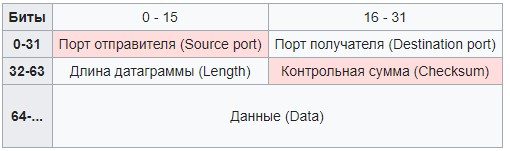
\includegraphics{./files/udp_header_scheme.jpg}
\caption{Заголовок сегмента UDP}
\end{figure}

Не требует установки соединения для передачи данных и тем самым не
гарантирует доставку пакетов и правильных их порядок. Используется в
ситуациях когда нужно принимать множество пакетов от разных
пользователей или когда потеря нескольких пакетов не критична.

\hypertarget{ux441ux43aux430ux43dux438ux440ux43eux432ux430ux43dux438ux435-ux43fux43eux440ux442ux43eux432-ux441ux43aux430ux43dux435ux440-ux43fux43eux440ux442ux43eux432}{%
\subsubsection{Сканирование портов (сканер
портов)}\label{ux441ux43aux430ux43dux438ux440ux43eux432ux430ux43dux438ux435-ux43fux43eux440ux442ux43eux432-ux441ux43aux430ux43dux435ux440-ux43fux43eux440ux442ux43eux432}}

\textbf{Сканирование портов} - сканирование хоста или сети на наличие
открытых портов. ПО для сканирование портов называется \textbf{сканером
портов}. Так как программное обеспечение работающее по тому или иному
порту может иметь уязвимости, такой открытый порт может являться
серьезной угрозой информационной безопасности. В связи с этим сканерами
портов пользуются или системные администраторы для предотвращения атак
или злоумышленники для поиска точек входа в систему.
